%%%%%%%%%%%%%%%%%%%%%%%%%%%%%%%%%%%%%%%%%%%%%%%%%%%%%%%%%%%%%%%%
% Thesis proposal, University of Amsterdam 
% Lukas Snoek, lukassnoek@gmail.com
%
% The title-page template was downloaded from 
% latextemplates.com and adapted to fit the
% RMP thesis proposal form. 
%
% Original author title-page template:
% WikiBooks (http://en.wikibooks.org/wiki/LaTeX/Title_Creation)
% CC BY-NC-SA 3.0 (http://creativecommons.org/licenses/by-nc-sa/3.0/)
%
%%%%%%%%%%%%%%%%%%%%%%%%%%%%%%%%%%%%%%%%%%%%%%%%%%%%%%%%%%%%%%%%

%%%%%%%%%%%%%%%%%%%%%%%%%%%%%%%%%%%%%%%%%%%%%%%%%%%%%%%%%%%%%%%%
% START PRE-AMBLE
\documentclass[12pt,a4paper]{article}\usepackage[]{graphicx}\usepackage[]{color}
%% maxwidth is the original width if it is less than linewidth
%% otherwise use linewidth (to make sure the graphics do not exceed the margin)
\makeatletter
\def\maxwidth{ %
  \ifdim\Gin@nat@width>\linewidth
    \linewidth
  \else
    \Gin@nat@width
  \fi
}
\makeatother

\definecolor{fgcolor}{rgb}{0.345, 0.345, 0.345}
\newcommand{\hlnum}[1]{\textcolor[rgb]{0.686,0.059,0.569}{#1}}%
\newcommand{\hlstr}[1]{\textcolor[rgb]{0.192,0.494,0.8}{#1}}%
\newcommand{\hlcom}[1]{\textcolor[rgb]{0.678,0.584,0.686}{\textit{#1}}}%
\newcommand{\hlopt}[1]{\textcolor[rgb]{0,0,0}{#1}}%
\newcommand{\hlstd}[1]{\textcolor[rgb]{0.345,0.345,0.345}{#1}}%
\newcommand{\hlkwa}[1]{\textcolor[rgb]{0.161,0.373,0.58}{\textbf{#1}}}%
\newcommand{\hlkwb}[1]{\textcolor[rgb]{0.69,0.353,0.396}{#1}}%
\newcommand{\hlkwc}[1]{\textcolor[rgb]{0.333,0.667,0.333}{#1}}%
\newcommand{\hlkwd}[1]{\textcolor[rgb]{0.737,0.353,0.396}{\textbf{#1}}}%

\usepackage{framed}
\makeatletter
\newenvironment{kframe}{%
 \def\at@end@of@kframe{}%
 \ifinner\ifhmode%
  \def\at@end@of@kframe{\end{minipage}}%
  \begin{minipage}{\columnwidth}%
 \fi\fi%
 \def\FrameCommand##1{\hskip\@totalleftmargin \hskip-\fboxsep
 \colorbox{shadecolor}{##1}\hskip-\fboxsep
     % There is no \\@totalrightmargin, so:
     \hskip-\linewidth \hskip-\@totalleftmargin \hskip\columnwidth}%
 \MakeFramed {\advance\hsize-\width
   \@totalleftmargin\z@ \linewidth\hsize
   \@setminipage}}%
 {\par\unskip\endMakeFramed%
 \at@end@of@kframe}
\makeatother

\definecolor{shadecolor}{rgb}{.97, .97, .97}
\definecolor{messagecolor}{rgb}{0, 0, 0}
\definecolor{warningcolor}{rgb}{1, 0, 1}
\definecolor{errorcolor}{rgb}{1, 0, 0}
\newenvironment{knitrout}{}{} % an empty environment to be redefined in TeX

\usepackage{alltt}
\usepackage[utf8]{inputenc}
\usepackage{amssymb}
\usepackage[colorlinks=false,hidelinks = true]{hyperref}
\usepackage[capposition=top]{floatrow}
\usepackage{natbib}
\bibliographystyle{apalike}

\usepackage{setspace} 
\setlength{\parindent}{10mm}

\usepackage{graphicx}
\graphicspath{ {images/} }

% Header style
\usepackage{fancyhdr}
\pagestyle{fancy}
\fancyhf{}
\renewcommand{\headrulewidth}{0pt}
\lfoot{Graduate School of Psychology}
\rfoot{Page \thepage}
\IfFileExists{upquote.sty}{\usepackage{upquote}}{}
\begin{document}

%%%%%%%%%%%%%%%%%%%%%%%%%%%%%%%%%%%%%%%%%%%%%%%%%%%%%%%%%%%%%%%%
% Start titlepage environment
\begin{titlepage}

\newcommand{\HRule}{\rule{\linewidth}{0.5mm}} 
\center 

% Headings
\textsc{\LARGE Graduate School of Psychology}\\[1cm] 
\textsc{\Large University of Amsterdam}\\[1cm]

% Title section
\HRule \\[0.4cm]
{ \huge \bfseries Research Master's Psychology Thesis Proposal Form}\\[0.4cm] 
\HRule \\[1.5cm]
 
% Author section & version/data info
\begin{minipage}{0.4\textwidth}
\begin{flushleft} \large
\emph{Author:}\\
Lukas \textsc{Snoek} 
\end{flushleft}
\end{minipage}
~
\begin{minipage}{0.4\textwidth}
\begin{flushright} \large
\emph{Version:} \\
\textsc{1st draft} 
\end{flushright}
\end{minipage}\\[2cm]

% Logo

\includegraphics[width=60mm]{uva_logo3}\\[2cm] 

% Data
{\large \today}\\[3cm]

\vfill 

\end{titlepage}

%%%%%%%%%%%%%%%%%%%%%%%%%%%%%%%%%%%%%%%
% KNITR stuff



%%%%%%%%%%%%%%%%%%%%%%%%%%%%%%%%%%%%%%%%
% Texcount 
\newcommand\wordcount{
    \immediate\write18{texcount -sub=section \jobname.tex  | grep "Section" | 
    sed -e 's/+.*//' | sed -n \thesection p > 'count.txt'}
Word count: \input{count.txt}}

%%%%%%%%%%%%%%%%%%%%%%%%%%%%%%%%%%%%%%%%
% Begin actual proposal form
\onehalfspacing

\section{Who and Where?}
\vspace{\baselineskip}

\begin{tabular}{l l l}
\textbf{Student} \\
Name & : &                              Lukas Snoek\\
Student ID number & : &                 10126228 \\
Address & : &                           Commelinstraat 332 \\
Postal code and residence & : &         1093VD, Amsterdam \\
Telephone number & : &                  +31647769183 \\
Email address & : &                     lukassnoek@gmail.com \\[0.5cm]

\textbf{Supervisor(s)} \\
Within ResMas (obligatory) & : &            Dr. H.S. Scholte \\
Specialisation & : &                        Brain \& Cognition \\
External supervisor(s), if any & : &        n/a \\
Second assessor & : &                       Prof. dr. R. Ridderinkhof \\
Research center / location & : &            Spinoza centre for neuroimaging \\[0.5cm]

\textbf{Number of credits} & : &            28 \\
\textit{At least 25 ec} \\[0.5cm]

\textbf{Ethics committee reference code} & : & 2015-BC-4120 \\
\textit{https://www.lab.uva.nl/ce/} \\[0.5cm]

\end{tabular}

%%%%%%%%%%%%%%%%%%%%%%%%%%%%%%%%%%%%%%%%
\section{Title and summary research project}

\subsection{Title}
Contrasting dimensionality and spatial distribution between perceptual and emotional brain networks.

\subsection{Summary of proposal \textmd{- max 500 words}}
In the past decade, cognitive neuroscience witnessed a paradigm shift from functional localization to distributed representations of psychological processes in the brain. New analytical tools were developed to fill this methodological niche, including functional connectivity and multivariate modeling. Especially the latter technique, often known as Multivariate Pattern Analysis (MVPA), has shown to be a promising method to characterize and investigate distributed functional networks in the brain . Studies employing these multivariate analyses often claim to reveal a \emph{distributed} neural network representing a certain psychological process. In the psychological literature, however, the term "distributeness" has been used ambiguously and inconsistently, as multivariate representations may be present within a cluster of voxels, within a cortical lobe, or even across the entire brain \citep{coutanche2013}. For example, while object categories may be represented throughout the anterior temporal lobe \citep{haxby2001}, emotion networks seem to be represented across the entire brain \citep{lindquist2012}. Furthermore, given the spatial distribution of a psychological process, the question remains whether the representation is encoded within a distributed set of \emph{voxels} or within a distributed set of \emph{brain areas}. This study's proposal aims to investigate the spatial distribution and multivariate structure of two types of processes: perceptual processes, which are hypothesized to be distributed relatively locally in the ventral visual stream, and emotion-valence processes, which are hypothesized to be distributed brain-wide and within a set of brain areas rather than voxels. 

To investigate these hypotheses, we want to use functional magnetic resonance imaging (fMRI) to measure and contrast neural representations of object categories with neural representations of emotional valence. During fMRI acquisition, participants will be shown pictures of two exemplars of neural faces and two exemplars of visual scenes, embedded in an auditory narrative. Within the narrative, the pictures of neutral faces will be consistently associated with either positive or negative valence by characterizing the faces as the narrative's "hero" or "villain" respectively. The visual scenes are similarly coupled with either a positive or negative valence by portrarying one visual scene as a stereotypical "safe house" while the other scene is portrayed as the murder scene. This arrangement follows a factorial design (valence $\times$ object) in which the representation of object categories and valence can be investigated regardless of stimulus identity. In our analyses, we will
use multivariate encoding using a factorial MANOVA (see \citep{kornysheva2014}). With this analysis, we will be able to characterize and visualize perceptual and emotional networks in the brain in terms of their multivariate structure and spatial distribution. \\

\noindent
\wordcount

%%%%%%%%%%%%%%%%%%%%%%%%%%%%%%%%%%%%%%%%
\section{Project description \textmd{- max 1200 words}}
\subsection{Prior research}
% Describe prior research, a comprehensible literature review of the research field, % converging upon the research questions. 
%
% a) Describe the state of affairs, including the theoretical framework, in the   current research field based on the existing body of literature.
% b) Clarify how the previous research eventuates into the research questions of the current proposal

A key question in the field of cognitive neuroscience is how the brain represents information. The past decades, the neuroimaging literature was dominated by studies employing univariate analyses to investigate which brain areas (de)activate during a particular psychological process of interest. These analyses are considered to be univariate, as they model each voxel in the brain separately. Effectively, these types of studies aimed to localize psychological functions to particular brain areas. Consequently, researchers implicitly engaged in a type of "neo-phrenology" in which unique function-structure mappings were proposed \citep{poldrack2010}. For example, the amygdala became the "fear area" \citep{ledoux2003} and the anterior cingulate cortex became the "conflict area" \citep{vanveen2002}. In the light of our current understanding of the organization of the human brain, however, these function-structure mappings are unwarranted. First, for every purportedly selective function-structure mapping, several counter-examples exist \citep{poldrack2010}; second, and most importantly, significant (de)activation does not equal representation. In other words, the fact that a brain area activates in response to a certain stimulus does not mean that it represents (processing of) this stimulus.  

In the early 21st century, the cognitive neuroscience community gradually moved from this functional localization perspective to a more network-oriented perspective \citep{sporns2002}. Instead of asking \emph{what} regions (de)activate during a particular psychological process, they started asking \emph{how} brain areas or a network of brain areas encode and represent this particular process. Put differently, researchers shifted from a univariate to a multivariate analytic approach. One of the first studies to show that the human brain encodes psychological concepts as distributed -- multivariate -- representations was the seminal paper by \cite{haxby2001}. They showed that different object categories were represented in a distributed fashion across the ventral visual cortex, regardless of mean activation level. Their approach, for which they used the term Multivariate Pattern Analysis (MVPA), gained popularity quickly as it appeared to provide a more sensitive analysis as opposed to univariate analyses \citep{norman2006,haxby2012}. Several new multivariate analyses were developed in the succeeding years, including the (successful) application of machine learning classifiers to distinguish neural representations (e.g. \citealp{cox2003}) and representational similarity analyses to characterize relations between neural patterns in a continuous fashion \citep{kriegeskorte2008}. Currently, MVPA analyses are widespread in almost all domains of cognitive, affective, and social neuroscience. For example, in vision research, MVPA has been applied to correctly decode orientation preference at the voxel-level in striate cortex (\citealp{kamitani2005}, but see \citealp{opdebeeck2010} for a more nuanced interpretation).    

\subsection{Key questions}
% Now state the key questions, the essence of the proposal. Here, the intended research should be connected to prior research. Testable hypotheses should be derived from the key question, and the relation between theory and research hypotheses should be clearly specified.

% a) Formulate a general relevant research question based on previous research.
% b) Translate the general research question in a clear manner into a specific research question.
% c) Translate the specific research questions into testable research hypotheses.

\noindent
\wordcount 

%%%%%%%%%%%%%%%%%%%%%%%%%%%%%%%%%%%%%%%%
\section{Procedure \textmd{– approx. 1000 words}}
\subsection{Operationalisation}
% Describe how the research questions are operationalised. 
% a) Operationalise the research questions in a clear manner into a research design/strategy. 
% b) Describe the procedures for conducting the research and collecting the data. 

\subsection{Sample characteristics}
% a) Indicate, given a power analysis, how many participants will be recruited. Also motivate whether the resulting number is feasible.
In this study, we will apply both univariate and multivariate (RSA and MVPA) analyses. While for univariate analyses much is known about the optimal analysis parameters, this is less so for multivariate analyses due to the their novelty and fine spatial scale on which it operates. This warrants an approach in which various parameter settings -- e.g. smoothing kernel, feature selection methods, and ROI selection -- are tested for optimal use of the data. However, to avoid double-dipping the data, we implement the procedure originally proposed by \cite{kriegeskorte2009} (see figure 1) in which we partition the data set into an optimization-set and a validation-set. The data from the optimization-set will be used to explore various parameter settings, and when the optimal parameters are established, these will be cross-validated on the validation-set. This way, exploratory and confirmatory research can be combined to use the data optimally without double-dipping. 

This model cross-validation approach, however, comes at the cost of effectively cutting the experiment's power in half. As univariate analyses are generally less sensitive than multivariate analyses (e.g. smaller effect sizes due to stringent multiple comparison correction), the bottleneck in terms of power would be solely be determined by the univariate analysis. Fortunately, much more is known about the optimal parameters for univariate analyses. Therefore, to avoid the power bottleneck, we will perform the univariate analysis on the entire data set.

\begin{figure}[t]
\floatfoot{\textbf{Figure 1}: Schematic representation of the model optimization process for the multivariate analysis. A 50/50 partitioning ratio will be used. The univariate analysis will be done \emph{once} with predetermined parameter settings and will thus not be partitioned.}
\centering
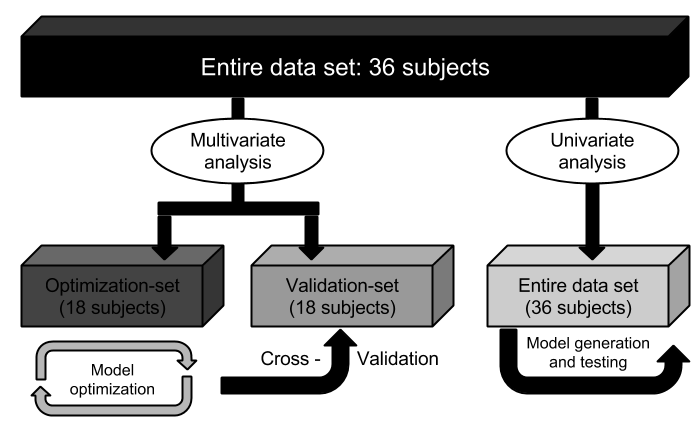
\includegraphics[scale=.5]{ModelOptimization}
\label{fig:figure1}
\end{figure}


% b) If a subset of participants will be excluded from the analysis given their scores on dependent variables, indicate the objective criterion to do so. For example include a phrase like: “Scores on dependent variables exceeding ± 3 sd of the mean will be excluded from the analysis’’
% c) If a subset of participants will be excluded from the analysis given their scores on a manipulation check item, indicate the objective criterion to do so. For example include a phrase like: “Participants scoring 15 or lower on a manipulation checks item, will be excluded from the analysis” 
% d) In case of a simulation study, indicate how data will be generated

\subsection{Materials}
% Indicate which tests, stimuli, equipment, etc. will be used; provide sufficiently elaborate descriptions and motivate your choice. (Always report the psychometric characteristics, such as reliability and validity, if existing tests are used. If new or adapted instruments or test materials (e.g., questionnaires) will be developed, then the new instrument must be independently validated first; only then it can be used as a testing instrument. Exception to this rule is allowed in case of questionnaires that do not contain more than one question (e.g., indicate on a 5-point scale how you feel today). 

\subsection{Data analysis}
% Indicate for each research question separately, how it is translated into a statistical prediction. For example: “In a repeated measures ANOVA we expect an interaction effect of the between factor x and the within factor y on the dependent variable z. Also indicate how you will correct for multiple comparisons. Only the analyses proposed here can be described as confirmatory analyses in your research report. All other have to be mentioned as exploratory. 

\subsection{Modifiability of procedure}
% Is there room for modification of the intended procedure? Evaluation of the proposal by the RMP Thesis Committee is meaningful only if the recommendations that the Committee might have can be implemented. It is therefore required that the intended procedure can be modified before you start gathering data. In situations where procedures or operationalisations or sample characteristics cannot be modified, the Thesis Committee has to be consulted before handing in the research proposal. The committee will consider the eligibility of this project for a research thesis. 
The research project as proposed here can be modified along recommendations from the RMP Thesis Committee and others, in each stage of the project (preparation/stimulus materials, data acquisition, or analyses). Advice on any section of this project is very much appreciated. \\

\noindent
\wordcount

%%%%%%%%%%%%%%%%%%%%%%%%%%%%%%%%%%%%%%%%
\section{Intended results \textmd{- max 250 words}}
% Clarify what the implication of possible outcomes would be (per hypothesis) for the specific and general research questions as well as for the theory. Address the following in approximately 250 words:

% a) What are the interpretations if the results do  match the expectations? 

% b) What are the interpretations if the results do not match the expectations?

% c) Are there any alternative interpretations?

% d) Is there any practical or societal relevance? Please explain. 

\noindent
\wordcount

%%%%%%%%%%%%%%%%%%%%%%%%%%%%%%%%%%%%%%%%
\section{Work plan \textmd{– max 500 words}}
% Describe how the research project will be executed. Who is doing what and when? Is the planning of the current project realistic, efficient and feasible?
The research project can be conceptually divided into three stages. The preparation stage, spanning from March to mid April, will be centered around gathering the necessary stimulus materials and programming the Presentation script. This will be done in collabroration with Steven Scholte. Suzanne Oosterwijk will additionally aid in this stage because of her expertise in emotion research. In this stage I will also start programming a fully open-source preprocessing and analysis pipeline in Python, with a focus on "literate programming" \citep{knuth1984}, transparancy, and reproducibility (as argued here: \url{http://tinyurl.com/pmveewc}). Tomas Knapen (VU University), who is very experienced Python programmer, will assist in creating the pipeline. Early April I will begin recruiting participants. 

The data acquisition stage will start mid April, when the 3T scanner at the Spinoza Centre for Neuroimaging will be fully operational again after the hardware upgrade. I plan to scan 36 participants in three weeks time. As the experimental protocol takes about 40 minutes, this will result in 8 hours per week. If there is more time available at the scanner, I will try to scan more people per week. During this stage, I will start programming the multivariate encoding analysis. Steven Scholte and Renée Visser (who is experienced with RSA analyses) will help with programming the analysis.

In the first or second week of May (depending when data acquisition is finished), the data analysis stage will start. This stage will be centered around finishing the analysis scripts and subsequently trying out different parameters on the optimization-set. In the first week of June, I hope to execute the final analysis on the validation-set and start writing my thesis report. I plan to finish a draft of my report mid July and, after revision, submit a final version at the end of the month.

\subsection{Time schedule}
% State the total amount of ec as noted in the thesis contract (25-31 ec excl. proposal), 1 ec stands for 28 hours work. Present and justify a time schedule in weeks, including your time investment in hours per week. Plan some spare time, and indicate what elements can be cut / reduced if necessary.
The project will amount to a total of 28 EC, or  784 hours. Assuming a standard 40 hours (5 day) working week, the research project will be finished the 24th of July. This allows for one week of planned vacation. In case of unplanned delay in either stage of the research project, the parameter optimization process can be shortened. 

\subsection{Infrastructure}
% Where will the research take place? How is access to the facilities and materials ensured?
Data acquisition will take place at the Spinoza Centre for Neuroimaging. As a research assistant, I have access to the centre and its facilities at all times. The centre provides all necessary equipment, including proprietary software (e.g. Presentation). 

\subsection{Budget}
% The compensation from the department is max € 80 for each research project. If the total expenditure exceeds the maximum compensation, then specify how the surplus will be financed. The € 80 budget may be used for printing costs (e.g. for the conference poster), travel expenses, participant payment. Specify the financial ramifications for the intended research. Please go to the secretariat of the specialization of your supervisor with your receipts. The secretariat will reimburse the costs you made up to € 80. 
The research project will be financed by funds of Steven Scholte. I will use approximately 30 euros of the Brain \& Cognition departemental budget to print a poster which I will present at the annual Research Master's Graduate Conference. \\

\noindent
\wordcount

%%%%%%%%%%%%%%%%%%%%%%%%%%%%%%%%%%%%%%%%
% Bibliography, natbib with apalike style 
\renewcommand{\bibsection}{} % Turn off header creation
\section{References}
\bibliography{refs}
% List all cited literature, formatted according to the directions of the APA Manual.

%%%%%%%%%%%%%%%%%%%%%%%%%%%%%%%%%%%%%%%%
\section{Further steps}
Make sure your supervisor submits an Ethics Checklist for your intended research to the Ethics Committee of the Department of Psychology at http://ce.psy-uva.nl/. Submit the research proposal in PDF by email to researchmaster-psychology@uva.nl. 
If you have the proposal signed by the supervisor(s) and you have scanned their signatures in the PDF, you only have to hand in a digital version of the proposal. However if the signatures are not on the PDF, please also submit a printed copy of the signed research proposal to the secretariat of the Research Master Psychology:
\vspace{\baselineskip}

\noindent
Universiteit van Amsterdam \\
Research Master’s Psychology \\
Weesperstraat 4, room 1.02 \\
1018 XA Amsterdam \\
researchmaster-psychology@uva.nl
\vspace{\baselineskip}

\noindent
A response of the Research Master's Thesis Committee can be anticipated within 10 workdays (i.e. two weeks) after handing in the proposal. 

%%%%%%%%%%%%%%%%%%%%%%%%%%%%%%%%%%%%%%%%
\section{Signatures}
$\square$ I hereby declare that both this proposal, and its resulting thesis, will only contain original material and is free of plagiarism (cf. Chapter 11 or the Research Master's course catalogue).
\vspace{\baselineskip}

\noindent
$\square$ I hereby declare that the result section of the thesis will consist of two subsections, one entitled "confirmatory analyses" and one entitled "exploratory analyses" (one of the two subsections may be empty):

\begin{enumerate}
\item The confirmatory analysis section reports exactly the analyses proposed in section 4 of this proposal
\item The exploratory analysis section contains additional, and thus exploratory, analyses. 
\end{enumerate}

\noindent
\textbf{Signature student:} 
\vspace*{2\baselineskip} \\
\line(1,0){175} \\

\noindent
\textbf{Signature ResMas supervisor:}
\vspace*{2\baselineskip} \\
\line(1,0){175} \\

% Uncomment if you have an external supervisor
%
%\textbf{Signature external supervisor (if applicable):}
%\vspace*{2\baselineskip} \\
%\line(1,0){175} \\

\end{document}
